\label{openmp}
OpenMP stands for Open Multi-Processing. OpenMP is an Application Programming Interface (API) to facilitate parallel programming  on shared memory systems. \citep{chapman08}  It is a set of compiler directives and supporting callable runtime library routines and environment variables that extends C/C++ and Fortran to express shared memory parallelism. \citep{dagum:98}

In 1990's OpenMP was defined by OpenMP Architecture Review Board (ARB), formed by a group of leading Hardware and Software vendors to provide a common API for programming a range of SMP architectures. This was based on earlier similar work done by Parallel Computing Forum(PCF). Unlike MPI which we will discuss below, OpenMP is not a standard. Instead, it is considered as an agreement between members of ARB who shares common interest in portable, user-friendly and efficient approach to shared memory parallel programming. \citep{chapman08}
OpenMP API was designed to provide an easy method to thread application without requiring a programmer to know how to create threads, synchronise and destroy them or even how many to create.

OpenMP does not define a new language. It is a set of compiler directive that can be added to a sequential  program to describe how a work can be shared among threads executing on different processor cores and synchronise their access to shared data if needed. These compiler directives make it easy to modify a sequential program to take advantage of  shared-memory parallel architecture with a minimum modification to existing codes.
OpenMP is simple to use because the complexity of parallelism is handled by the compiler and also it emphasised on structured parallel programming. \citep{chapman08}

\subsubsection{Thread based parallelism}
OpenMP is based on Multithreading. Program launches as a single thread which can create other threads if required. It utilises the "fork" and "join" model of parallel execution.  All OpenMP program starts as a single process which is known as master thread. The master thread continues the program execution sequentially to the point where it encounter a parallel region of the program defined by a OpenMP construct directive. \citep{Barney:16-openmp}

\begin{figure}[!htb]
	\centering
	\begin{subfigure}[b]{\textwidth}
  		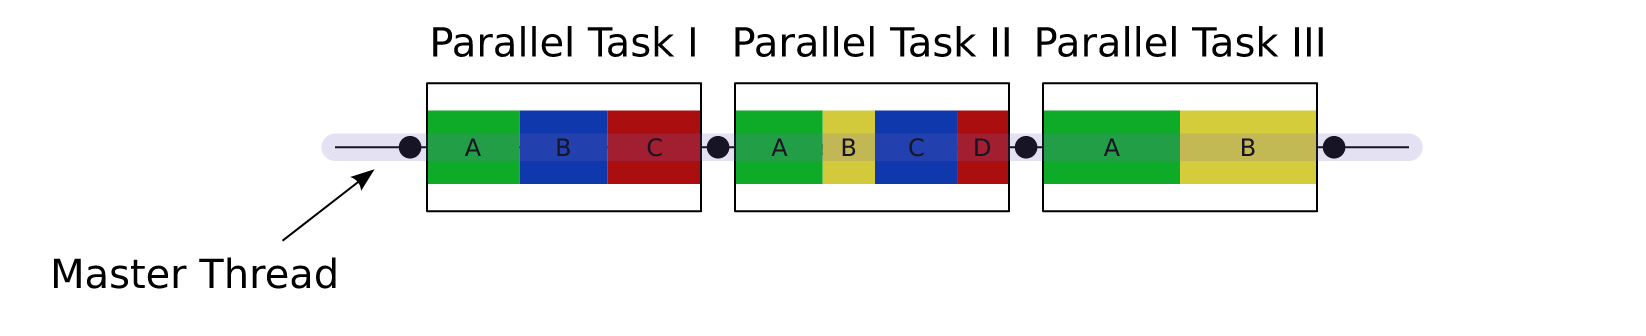
\includegraphics[width=\textwidth]{figs/fork_join_a.png}
  		\caption{Sequential execution: All of the Parallel Task blocks are executed by a single thread(Master).}
  		\label{fig:fork_join_a}
	\end{subfigure}
	\begin{subfigure}[b]{\textwidth}
  		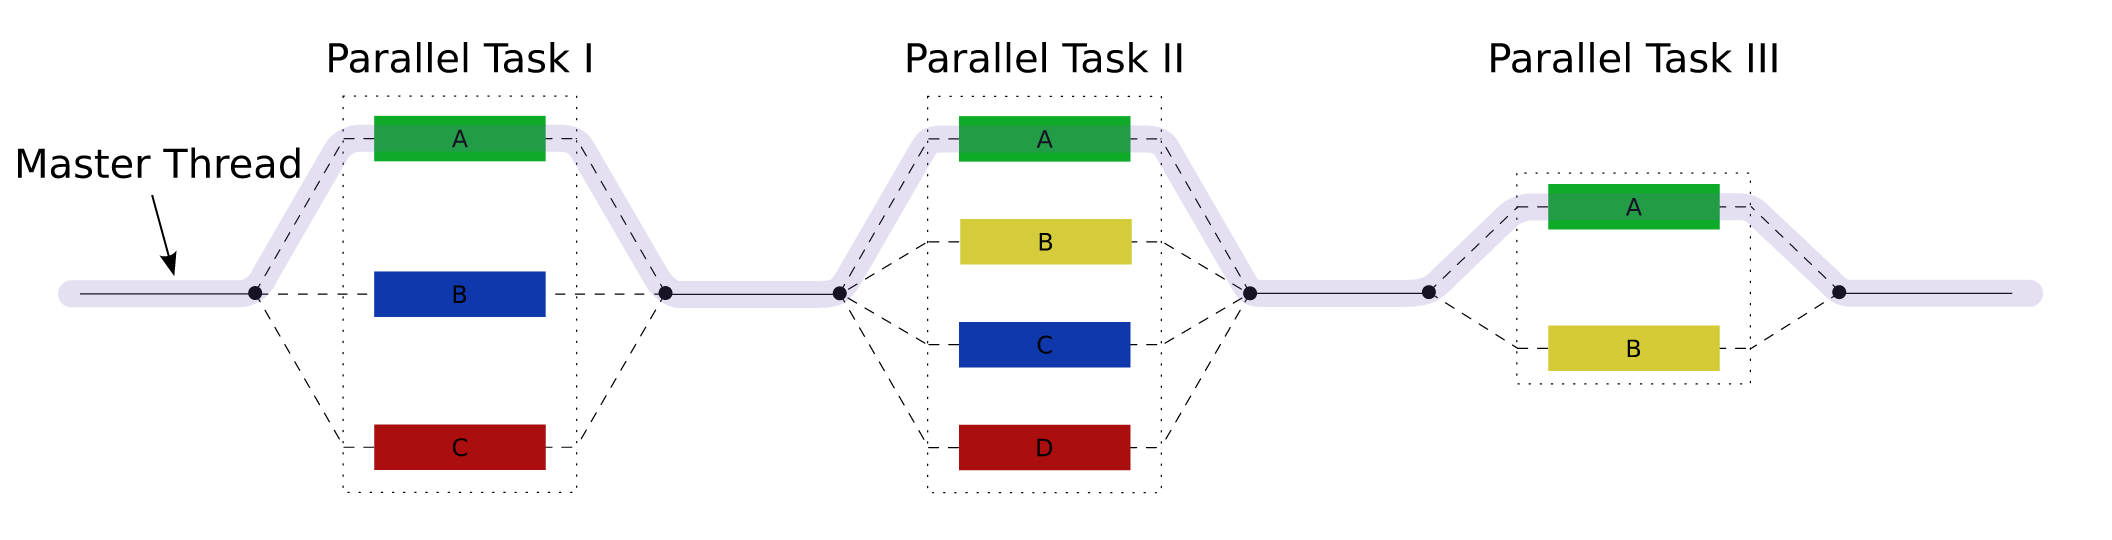
\includegraphics[width=\textwidth]{figs/fork_join_b.png}
  		\caption{Parallel execution: At each Parallel Task block the master thread forks multiple team threads which then execute the subtasks within that parallel region concurrently.  When finished the team threads then join with master thread and terminate before master thread advancing to the next parallel region.}
  		\label{fig:fork_join_b}
	\end{subfigure}
	\caption{Fork- Join model. \citep{A1:fork-join}}
  	\label{fig:fork-join}
\end{figure}

In Figure \ref{fig:fork-join} shows the fork-join model of parallel execution. It shows a program containing parallel executable code fragments. These code fragments are put into three region labelled as \textbf{Parallel Task I, Parallel Task II and Parallel Task III} to show the synchronisation points. Within these points program must synchronise before advancing. Each group contain code fragments of subtasks (labelled as A, B, C, D etc.) that are independent of each other and can be executed in parallel asynchronously. These subtasks can take advantage of concurrent execution by multiple threads. Figure \ref{fig:fork_join_a} shows the program is executed by a single thread(Master thread). The Figure \ref{fig:fork_join_b} shows that the same program is parallelise using fork-join model. When master thread reaches a parallel region it forks multiple team threads as required by that region. These team threads then execute the subtasks (A, B, C, D etc.) assigned to them concurrently. When the team threads complete executing the subtasks, they join back to the master thread and terminate. The master thread is then continue with rest of the program.

\subsubsection{OpenMP Components}
The OpenMP API comprised of three primary components:
\begin{itemize}
	\item Runtime Library Routines
	\item Environment Variables
	\item Compiler directives
\end{itemize}

\subsubsection{Runtime Library Routines}
The Runtime library routines are used for setting up  and identifying number of threads, thread numbers for identification, dynamically adjusting of threads, timers, nested parallelism and for locking mechanism. \citep{Barney:16-openmp}

\subsubsection{Environment Variables}
OpenMP provides several environment variables for controlling the execution of parallel code at runtime. These variables can be used to control the number of threads, scheduling type, binding threads to processor, controlling level of nested parallelism, dynamic thread adjustment, stack size and thread wait policy. \citep{Barney:16-openmp}


\subsubsection{Compiler Directives}
Compiler directives are special constructs that specify how a compiler should process its inputs. OpenMP API uses compiler directives for C, C++ and Fortran compilers for marking a parallel region, distributing works among threads, dividing up loop iterations, serialising section of codes and for synchronisation of the work. In C/C++ source code the directives appears as \#pragma as shown at Line 2 of Listing  \ref{lst:openmp_format}. \citep{Barney:16-openmp}

\begin{lstlisting}[language=C, caption={OpenMP directive format in C/C++}, label={lst:openmp_format}]

#pragma omp <directive-name> [clauses, ...] newline

\end{lstlisting}

Using OpenMP compiler directives a programmer instructs the compiler which part of program to run in parallel and how to divide the work among threads that  will run it. These directives are meaningful to the compilers only. OpenMP directives looks like comments in Fortran programs and pragma in C or C++ program. The advantage of such implementation is that a program containing OpenMP directives will still compile and run even if a compiler is unable to interpret these directives.

The line 5 in "Hello world" program showing in Listing \ref{lst:helloworld} is a compiler directive in C program that marks the region as a starting point of the parallel execution.

\begin{lstlisting}[language=C, caption={A "Hello world" program in C using OpenMP compiler directive}, label={lst:helloworld}]
#include <stdio.h>

int main(void)
{
    #pragma omp parallel
    printf("Hello, world.\n");
    return 0;
}
\end{lstlisting}

OpenMP directives can be classified in following categories:
\begin{itemize}
	\item Parallel region construct
	\item Work-sharing constructs
	\item Synchronisation constructs
	\item Data-scoped attribute clauses
\end{itemize}

\paragraph{Parallel region construct} A parallel region is a block of code that will be executed by multiple threads. This construct forks additional threads to carry out the work within the next parallel code block. Line 5 in Listing \ref{lst:helloworld} shows the parallel directive that specifies a parallel region \citep{Barney:16-openmp}

\paragraph{Work-sharing constructs}
A work-sharing construct specify how independent work to be assigned to one or more threads. The \emph{omp for} and \emph{omp do} is used to divide up loop iteration among multiple threads. The \emph{section} clause is for assigning non-iterative consecutive but independent code blocks to multiple threads. The \emph{single} clause specify that a code block is to be executed by only one single thread. A code block to be executed only by master thread the \emph{master} clause is used. Listing \ref{lst:openmp_for} shows an example of \emph{for} work-sharing construct. \citep{Barney:16-openmp}

\begin{lstlisting}[language=C, caption={An example of Work-sharing "for" loop construct.}, label={lst:openmp_for}]
 #include <omp.h>
 #define N 1000
 #define CHUNKSIZE 100

 main(int argc, char *argv[]) {
 int i, chunk;
 float a[N], b[N], c[N];

 /* Some initializations */
 for (i=0; i < N; i++)
   a[i] = b[i] = i * 1.0;
 chunk = CHUNKSIZE;
 #pragma omp parallel shared(a,b,c,chunk) private(i)
   {
   #pragma omp for schedule(dynamic,chunk) nowait
   for (i=0; i < N; i++)
     c[i] = a[i] + b[i];
   }   /* end of parallel region */ 
 }
\end{lstlisting}

\paragraph{Synchronisation constructs}
OpenMP provides synchronisation constructs to deal with race-condition to ensure that the correct results is produced. The synchronisation constructs are used to control how the execution of each thread progress in relation to other threads. The example in Listing \ref{lst:openmp_critical} shows the use of Critical directive to define a critical region a program. \citep{Barney:16-openmp}

\begin{lstlisting}[language=C, caption={An example of Critical directive construct.}, label={lst:openmp_critical}]
#include <omp.h>

main(int argc, char *argv[]) {
 int x;
 x = 0;
 
 #pragma omp parallel shared(x) 
   {
   #pragma omp critical 
   x = x + 1;
   }  /* end of parallel region */
}
 \end{lstlisting}

\paragraph{Data-scoped attribute clauses}
As OpenMP is shared-memory model of parallelisation, most variables are are shared among multiple threads. OpenMP provides number of clauses to deal with variable scopes to define their visibility. These clauses are used in conjunction with other directives to control the scope of enclosed variable within a parallel code block. \citep{Barney:16-openmp}

\subsubsection{Advantages \& Disadvantages of OpenMP}
\paragraph{Advantages}
The following are the advantages and disadvantages of OpenMP as discussed on Dartmouth  College website on parallel programming. \citep{Dartmouth:mpi}.
\begin{itemize}
	\item Good performance and scalability
	\item OpenMP programs are portable
	\item Easier to program and debug compared to MPI
	\item Allow program to be parallelised incrementally
\end{itemize}

\paragraph{Disdvantages}

\begin{itemize}
	\item Can only be run in Shared-memory computers
	\item Requires compiler that supports OpenMP
	\item Mostly used for loop parallelisation
\end{itemize}

